\chapter{Application Design}
\label{cha:design}

After defining the mechanisms which will be implemented, in a next step, the general application flow will be described, as well as offering insight into the user experience design of all parts of the application. What is important to note is that the design discussed here is just the default layout and can easily be changed and adapted by the presenter. All features identified in chapter \ref{cha:mechanisms} can be turned on or off, in the following it is assumed that all of them are enabled.

\section{Application Flow}
The flow and usage of the application is separated into two parts: the creation and authoring of the presentation and giving the presentation. As the technical details of how slide decks are composed are covered in chapter \ref{cha:implementation}, this chapter focuses on the user interface and interaction design of the software from the speaker's and the audience's perspective, during the presentation.

The typical setup of an unveil presentation is as follows: We assume a presenter called Amy, who has already prepared her presentation and a listener called Greg who wants to follow the presentation from his smartphone.
The slides are generally served from a server. This can either be a publicly accessible server or, if all participants are in the same network, locally from Amy's computer. We assume Amy is serving the slides from her laptop, which is connected to a projector.
At the beginning of the presentation, Greg and all other listeners navigate their personal devices' browsers to the set up address (usually a combination of IP address and port). To make this step easier, Amy has put a QR code pointing to the address on the first slide and sent out an e-mail with the link to all participants before the start of the presentation.

The software supports three different modes out of the box: listener, speaker and projector mode. Depending on the mode, a certain set of features is activated, allowing Amy to have a different interface and more controls than Greg. Modes are activated via query parameters in the url: Amy navigates her laptop's browser to the url of the presentation and adds the query parameter \texttt{mode=projector}. On her smartphone, which she wants to use for remote controlling the presentation, the mode is set to \texttt{speaker}. If no query parameter is given, the application defaults to the listener mode, so Greg simply types in the address or follows the link in the url or QR code. Unveil generally offers a two-dimensional slide space, consisting of master slides (left to right) and subslides (top to bottom). Devices in speaker mode (in this example Amy's smartphone) can remote-control the presentation and navigate through said slides. All other devices (the laptop in projector mode and Greg's phone) are synchronised with the state of Amy's phone and automatically follow along in real-time.

% Base CSS: responsive, if content is too big, everything is uniformly scaled.

% Application Flow, Modes, How does the application work in general?
% Design aspects, sketches, wireframes, thoughts and überlegungen behind design details

\section{General Interface}
The general requirement for the interface of the application is to work in all three modes, on any device, from mobile phones to desktops and projectors. When in projector mode, only the content of the current slide, as well as listener reactions are shown (see figure \ref{fig:design-interface-projector}). In listener mode, the interface is a lot richer and additionally features buttons for sharing media, links and asking questions, as well as six different reactions (see figure \ref{fig:design-interface-listener}), which will be discussed in more detail in section \ref{sec:design-reactions}. It also offers small arrow buttons, to navigate between slides. The speaker interface is the most intricate: Besides showing the current slide, we believe it should also include a preview of the upcoming slides in $x$ (master slide) and $y$ (subslide) direction, as well as speaker notes. Additionally to this interface, already familiar from PowerPoint or similar presentation software, buttons to mute incoming requests (media, link and questions) and to create new polls are provided (see figure \ref{fig:design-interface-presenter}). Since we expect presenters to switch between devices more often than listeners for more typing-intense tasks such as creating new polls, the mobile interface is as similar as possible to the desktop one and only re-arranges the displayed information to fit on smaller screens. The main difference between the mobile and desktop version of the listener interface is the design of the reactions: While desktop computers and tablets offer ample space for the placement of all six emoji, these are hidden behind a button in the mobile interface and only slide up upon a tap on said button.

\begin{figure}
\centering
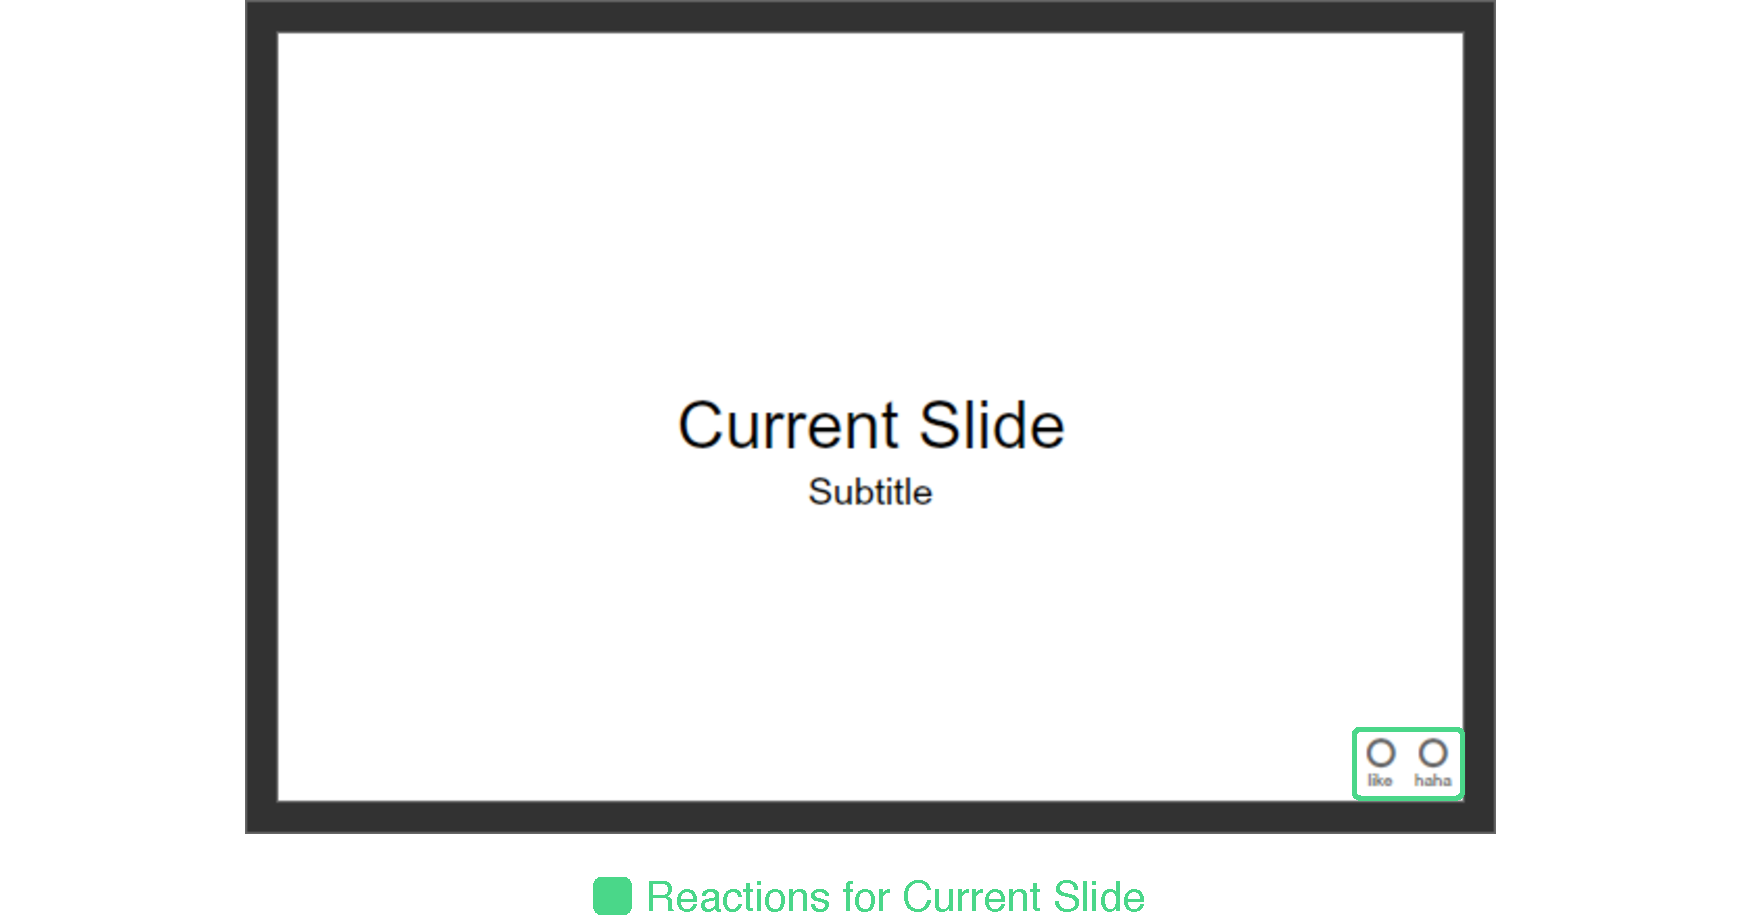
\includegraphics[width=.65\textwidth]{wireframes/projector-interface}
\caption{Wireframe of slide in projector mode, as seen on a projector. No visual controls are shown, only the current slide and listener reactions are displayed. The presentation progresses through the presenter mode's remote controlling feature.}
\label{fig:design-interface-projector}
\end{figure}

\begin{figure}
\centering
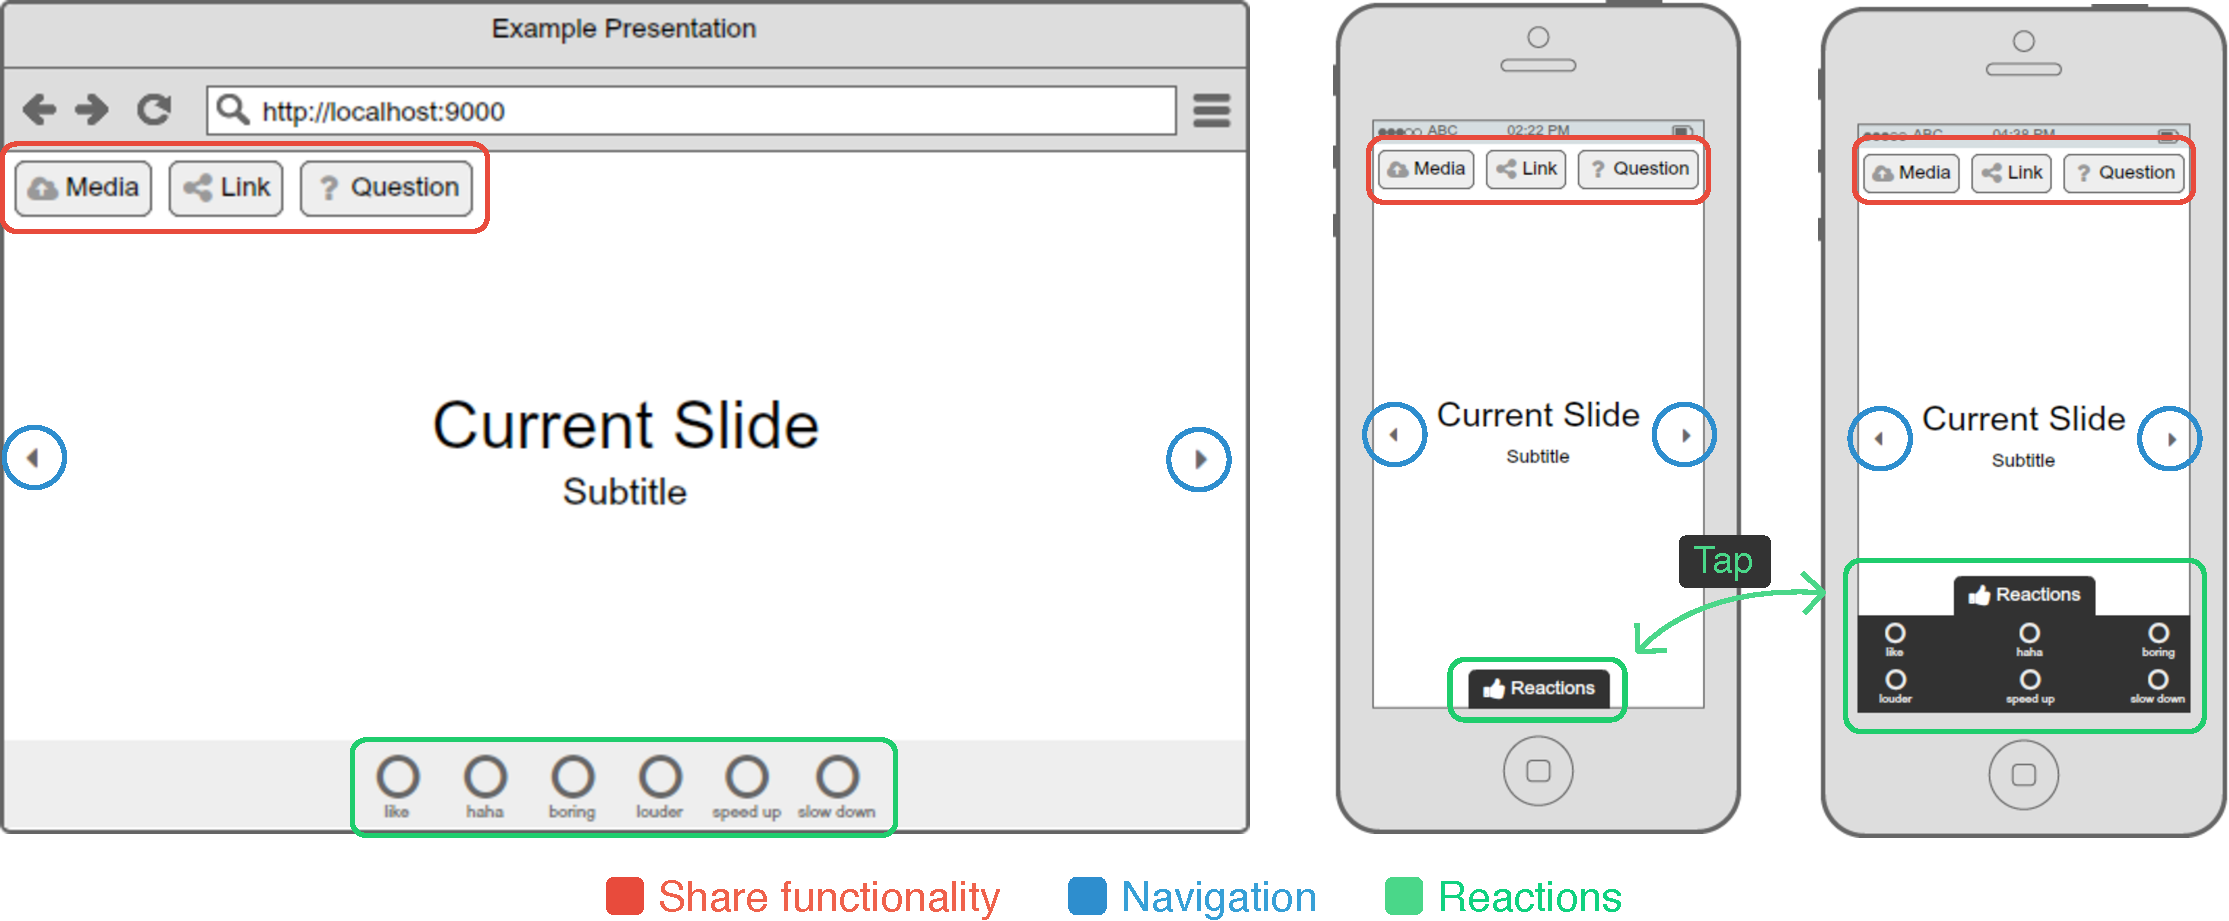
\includegraphics[width=.831\textwidth]{wireframes/listener-interface}
\caption{Wireframes of general interface in listener mode for mobile phones and desktops. Both offer buttons to share media, links and questions with the presenter, arrow buttons to navigate through the presentation and a possibility to react to the current slide. On mobile this feature is revealed with a tap on the \emph{reaction} button, to not cluster the interface.}
\label{fig:design-interface-listener}
\end{figure}

\begin{figure}
\centering
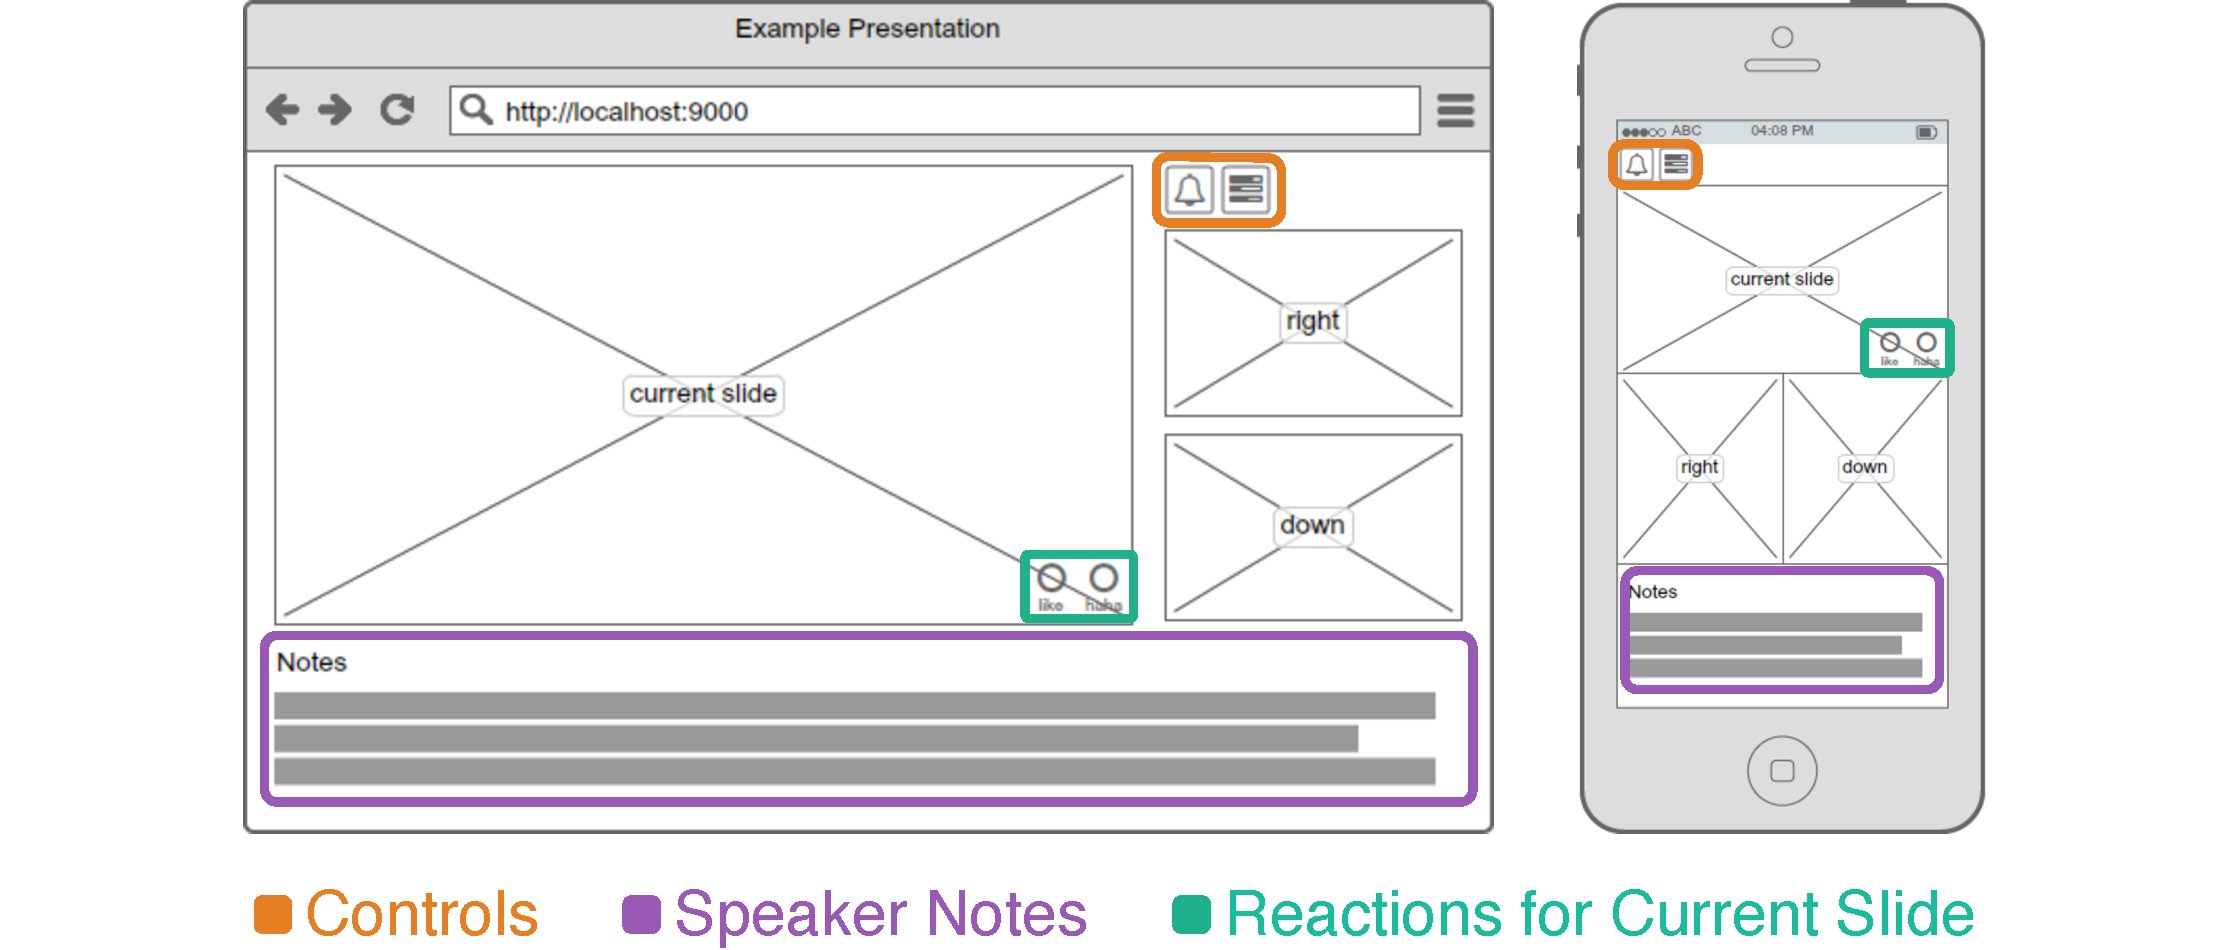
\includegraphics[width=.65\textwidth]{wireframes/speaker-interface}
\caption{Wireframes of general interface in speaker mode for mobile phones and desktops. The interface consists of a preview of the current slide, the next main slide (\emph{right}) and the next subslide (\emph{down}), as well as showing presenter notes. It also offers buttons to toggle muting of incoming requests and creation of new polls.}
\label{fig:design-interface-presenter}
\end{figure}

\begin{figure}
\centering
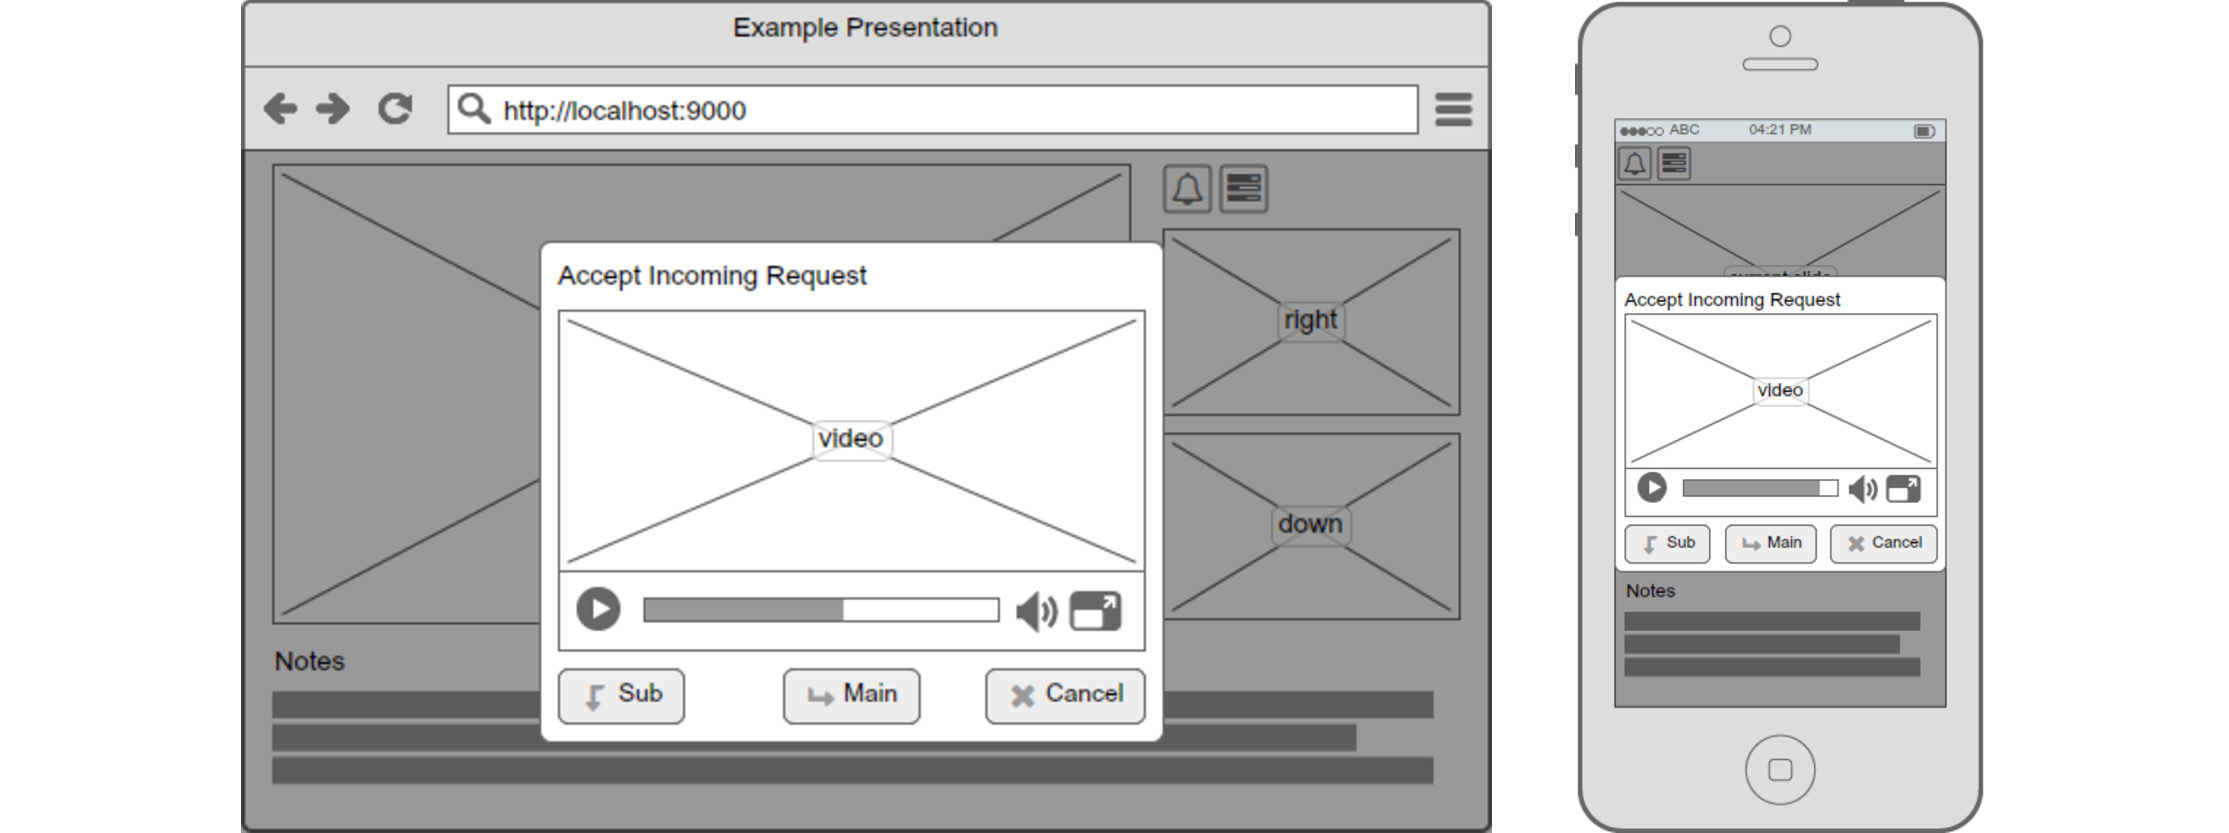
\includegraphics[width=.65\textwidth]{wireframes/modal-interface}
\caption{Wireframes of modal interface in speaker mode for mobile phones and desktops. The shown modal allows the presenter to add a listener-submitted video as a new main or subslide or dismiss the request. It pops up as soon as a listener wants to share content with the slide.}
\label{fig:design-interface-modal}
\end{figure}

\section{General Interaction Principles}
As far as the interaction design of the application is concerned, the main requirement technically is for all state changes to take immediate effect or in other words, for the software to work in real-time. This is true for interactions with the server as well as all internal state changes within the application. All transitions and animations last $200$ms, a value which is both usable on mobile phones and desktops and, according to Google's Material Design Guide \cite{GoogleMaterialDesignGuide} ``fast enough that it doesn't cause waiting, but slow enough that the transition can be understood''. An easing curve with low outgoing and high incoming velocity is used.

The general aim for the interaction design of the application is to be as easy and intuitive to use as possible on any device, for both presenters and listeners. Especially the speaker's view has a lot of information to display and many ways of interacting with the interface. From the speaker's point of view, the main reason for negative presentation experiences stems from technical difficulties and problems \cite{Wacker:PresenterExperience}; we therefore decided to design a presenter interface similar to the one already known from PowerPoint, Keynote, Google Slides or reveal.js (see figure \ref{fig:design-interface-presenter}) and employ familiar visual metaphors and interaction mechanisms such as buttons and modals (see \ref{gifig:design-interface-modal}).

Another important consideration when it comes to mobile and desktop environments is the question of supported inputs. While mouse and keys are a natural and intuitive way of navigating through desktop applications, swiping gestures are faster, more accurate \cite{Lai:SingleHandedThumbInteraction} and require less time looking at the screen on mobile devices \cite{Negulescu:TapSwipeMove}, making them the ideal candidate for the remote-controlling feature. For this reason, additionally to providing visual arrow-buttons for navigation, arrow-keys and swipe gestures are also supported. The interaction with buttons is controlled by mouse clicks or taps, respectively and common visual metaphors are used to symbolises their state (pressed, hovered, disabled), as shown in figure \ref{fig:design-interface-button}.

Now that the general interaction principles are covered, a more detailed look is taken at the most interesting parts of the implemented features.

\begin{figure}
\centering
\begin{tabular}{ccc}
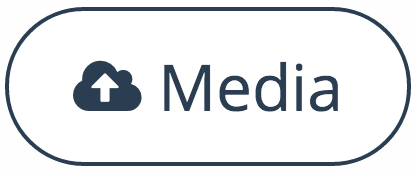
\includegraphics[width=.12\textwidth]{button-state-normal} &

\includegraphics[width=.12\textwidth]{button-state-hover} &
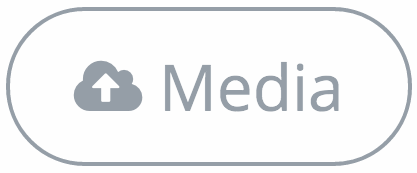
\includegraphics[width=.12\textwidth]{button-state-disabled} \\
(a) & (b) & (c)
\end{tabular}
\caption{Button states, (a) normal, (b) hovered or active and (c) disabled.}
\label{fig:design-interface-button}
\end{figure}

\section{Polls}
The first mechanism looked at in more detail is the polling feature. Polls can either be prepared before the start of the presentation or can dynamically be created during the presentation through the presenter interface. When Greg and the other listeners navigate through the presentation, they will already see the poll, they however cannot vote until Amy activates the voting by navigating to the slide with the poll. Polling again works in real-time: As soon as Greg chooses an option and presses the \emph{Vote} button, the presenter, projector and all listener interfaces will be updated with his vote immediately. Every listener is only allowed to vote once per poll and the only currently supported poll type is single-choice (see figure \ref{fig:design-polls}). As soon as Greg has voted, he is presented with the current results of the voting. These are displayed in horizontal bar charts (see figure \ref{fig:design-polls}), which are animated. This means, as soon as a new vote is registered, the bars will dynamically adjust their width as the percentages are updated. These results are available on the presenter and projector interfaces as well and also change in real-time.
While the voting is enabled (by Amy navigating to the slide with the poll and until she navigates away from it again), all other navigation is frozen. This means, in this time, all listener navigation is disabled to ensure everybody is on the same slide and exercises their right to vote; this, however, is not mandatory and listeners can also choose not to vote.

\begin{figure}
\centering
\begin{tabular}{ccc}
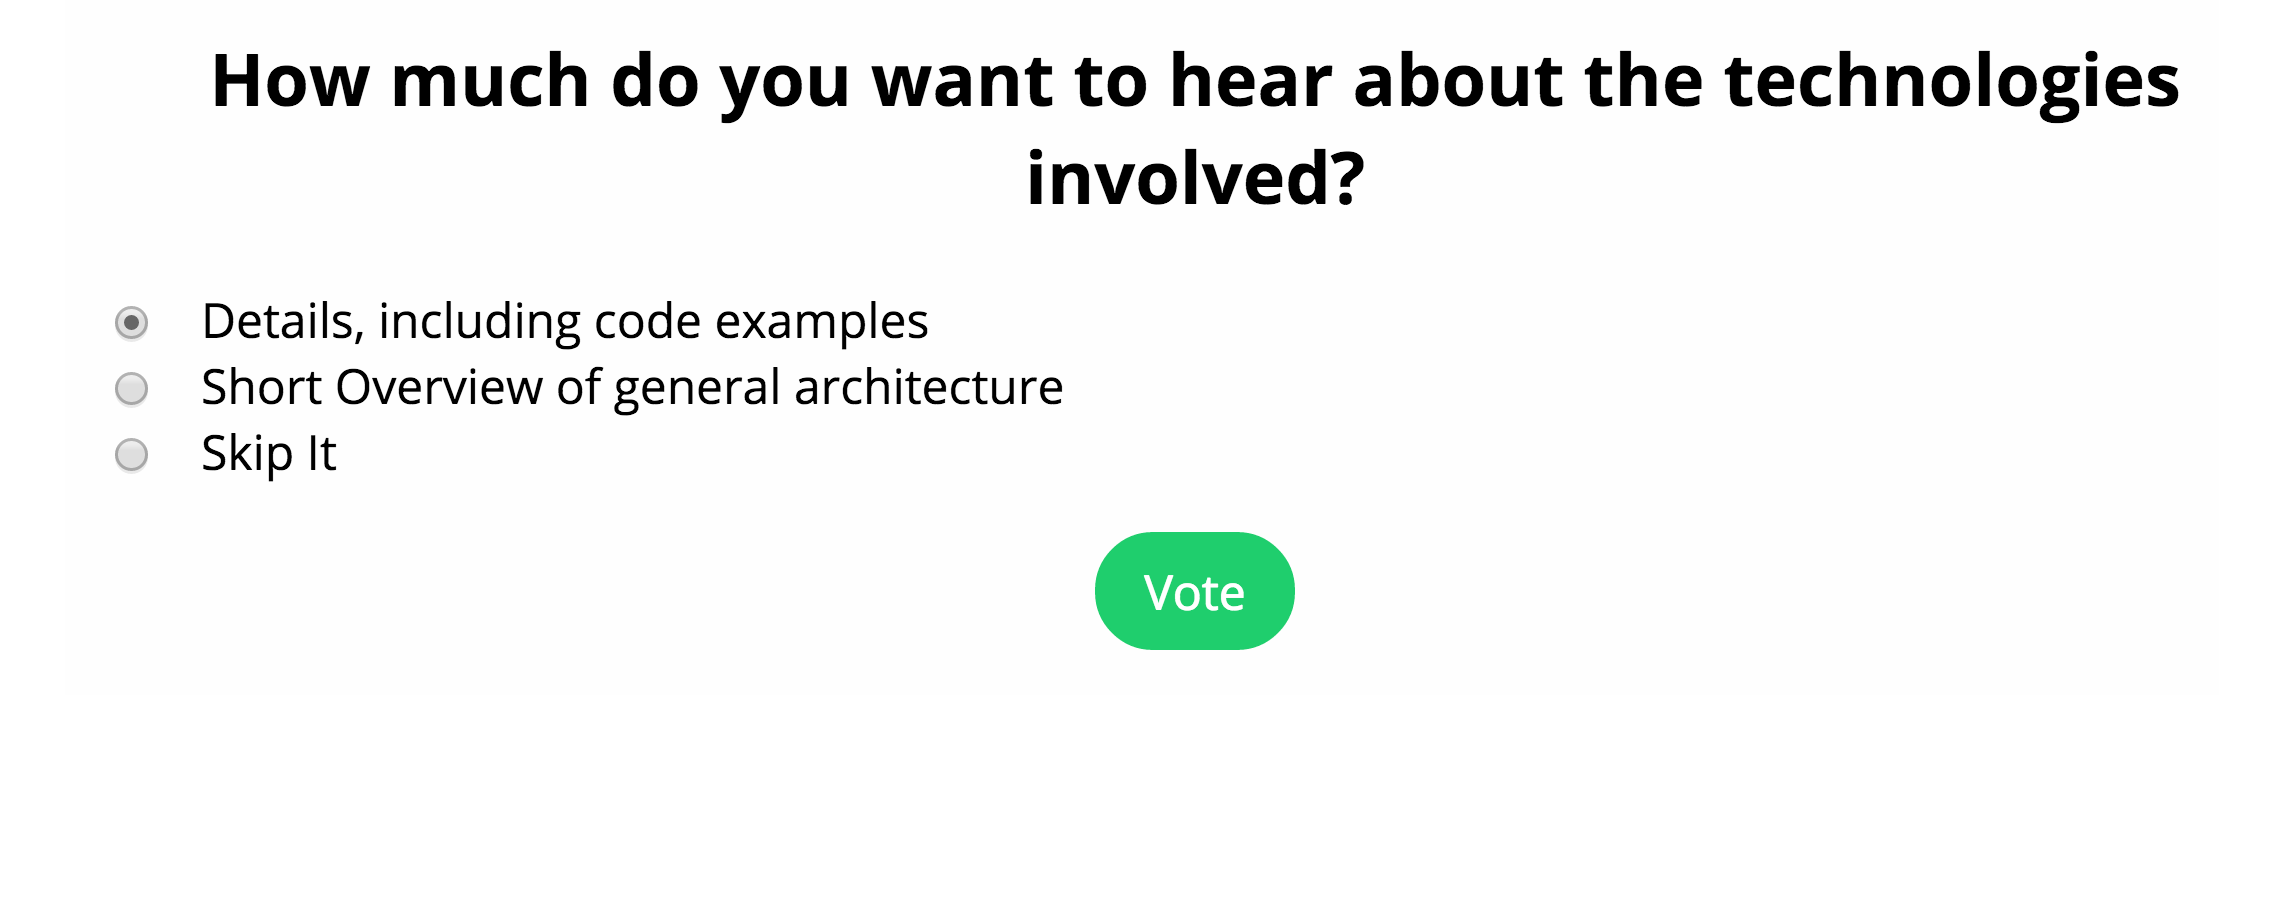
\includegraphics[width=.4\textwidth]{polls-voting} &
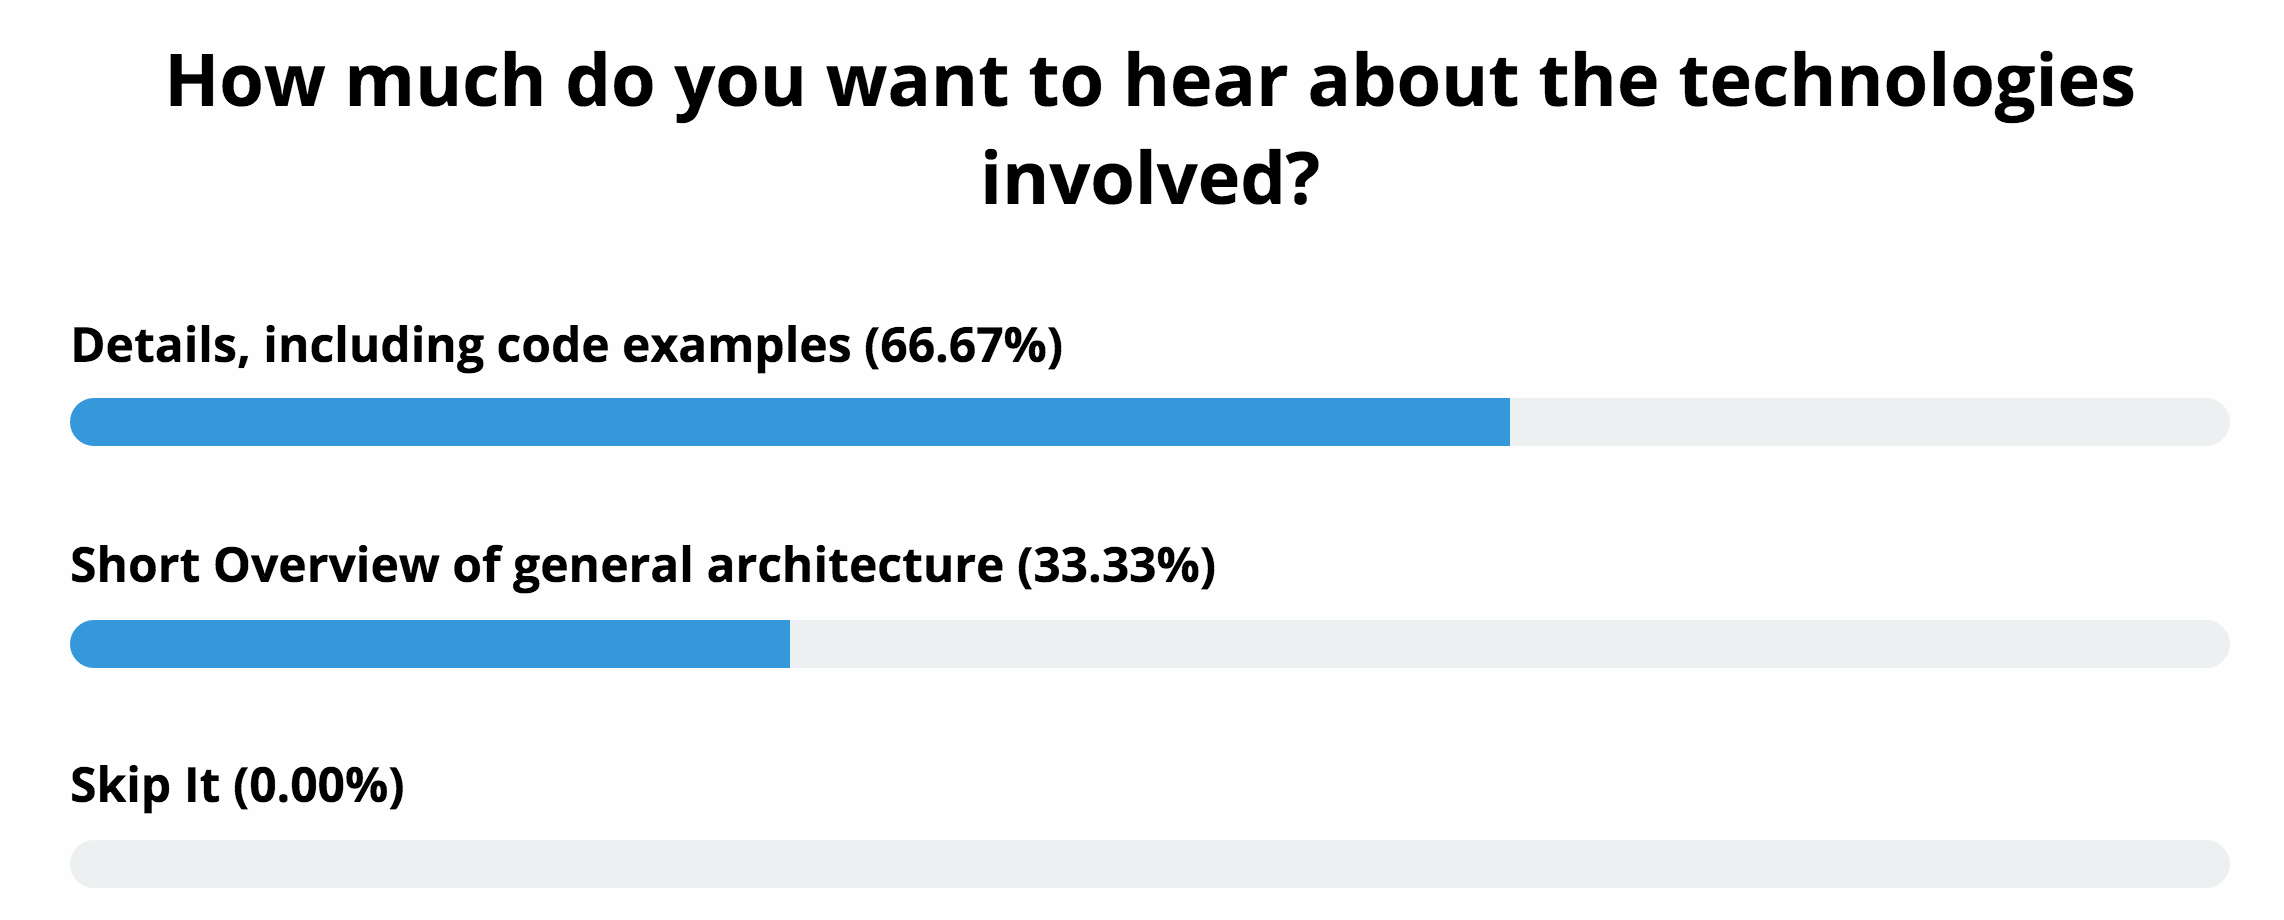
\includegraphics[width=.4\textwidth]{polls-results} \\
(a) & (b)
\end{tabular}
\caption{Details of polling interface for listeners before voting (a) and poll result after voting (b).}
\label{fig:design-polls}
\end{figure}

To create a new poll, the presenter presses or clicks the \emph{new poll} button in the controls section of the speaker interface, which opens a modal (see figure \ref{fig:design-polls-modal}). In the beginning, a question and two answer fields are provided, more answers can be added using the \emph{+} button. Once the question and answer options are entered, pressing the \emph{Create Voting} button will generate a new poll and add it as the next main slide.

\begin{figure}
\centering
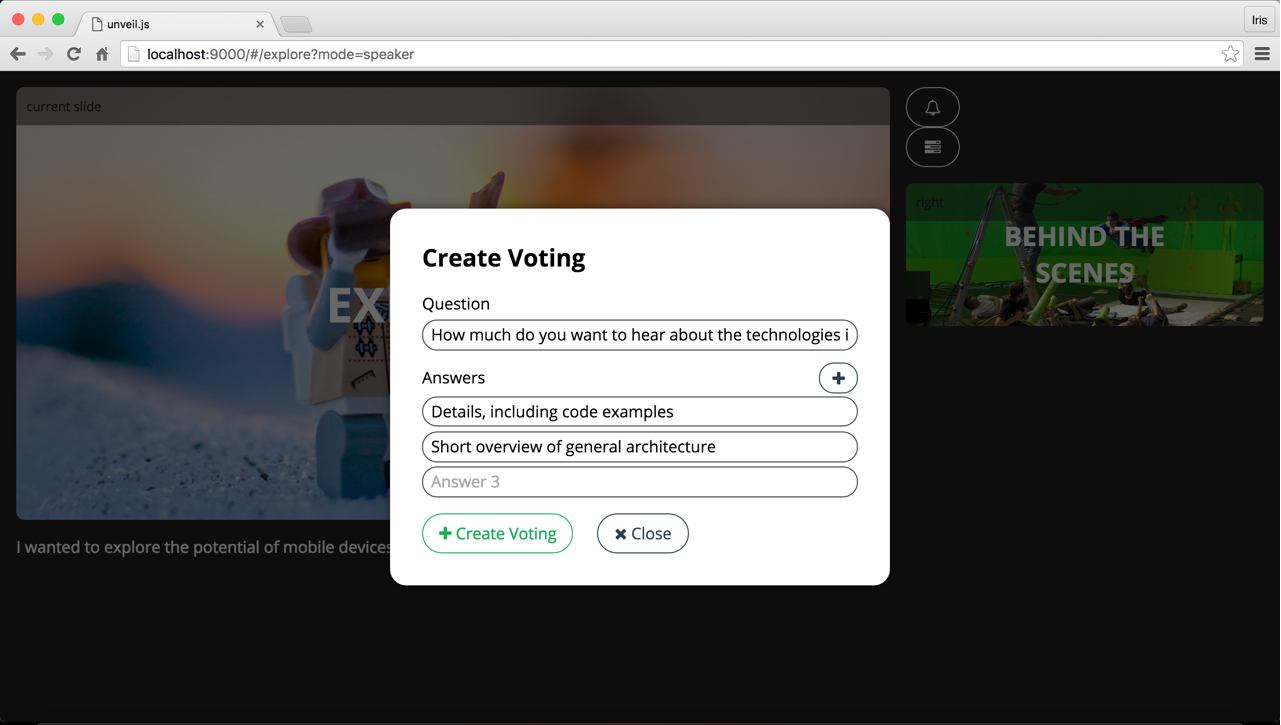
\includegraphics[width=.65\textwidth]{polls-modal}
\caption{Poll creation modal in presenter mode on tablets, laptops and desktops.}
\label{fig:design-polls-modal}
\end{figure}

\section{Reactions}
\label{sec:design-reactions}
% Emojis
% Find more studies about this! think: facebook, the conference Paulo went to etc. (maybe add photo of audience showing emoji faces!)
% It is therefore important to provide more detailed feedback. Following the evaluation in \cite{Teevan:MobileFeedbackDuringPresentation}, the mechanism proposed in this thesis offers three emotions (approval, laughter, boredom) and three request types (louder, speed up, slow down).
Although binary digital reactions in presentations are not an entirely new idea \cite{Teevan:MobileFeedbackDuringPresentation}, versatile feedback that goes beyond positive and negative, to our knowledge, has not yet been explored. The way this mechanism was implemented, our listener Greg can press a button to react to what the speaker Amy said or presented. The reactions are collected on a per-slide basis, allowing Amy to re-visit the slides afterwards, analysing which slides sparked most feedback. When Greg reacts to a slide, the feedback will immediately be displayed in the presenter view, as well as -- if enabled -- the projector interface.

Greg by default can choose from six pre-defined reactions: From the evaluation in \cite{Teevan:MobileFeedbackDuringPresentation} and \cite{Isaacs:InteractivePresentationsDistributedAudience} and from observing presentations and meetings, a pool of possible reactions has been narrowed down three emotions (approval, laughter, boredom) and three request types (louder, speed up, slow down) (see figure \ref{fig:design-reactions}). The reason behind the missing disapproval on one hand is that test subjects in \cite{Teevan:MobileFeedbackDuringPresentation} felt less comfortable giving negative feedback, the button was generally used less than the positive one and it also included feedback such as \emph{boredom} or \emph{speed up} and \emph{slow down}, which we have included own reactions for. On the other side, we hope this will encourage more elaborate feedback of disapproval using the content sharing functionality instead. This holds the potential of sparking a discussion instead of merely showing disagreement with the presented content.

The biggest challenge with displaying non-binary reactions was to find an intuitive and familiar visualisation which would not take up too much space on smaller screens. Since the introduction of emoji on Apple's keyboard in 2011 and on Android's one in 2013, emoji have become a ubiquitous, language-independent means of communication \cite{Instagramm:Emoji, Cappallo:ImageToEmoji}. Instagram has found that almost half of its comments and captions nowadays include emoji \cite{Instagramm:Emoji} and with Google \cite{Google:Emoji} and Bing \cite{Bing:Emoji} adding support for emoji-search and companies such as Facebook \cite{Facebook:Reactions} and GitHub \cite{Github:Reactions} offering emoji-based reaction systems, it is safe to assume the majority of regular internet users is familiar with the concept and meaning of emoji \cite{Cappallo:EmojiVideoSearch}. Although it would be possible to include a complete emoji-keyboard to allow for even more versatile feedback, we feel it is easier for less technology-oriented users to be provided only with a sub-set including a short description of each reaction (see figure \ref{fig:design-reactions}). However, it is worth noting that this sub-set can easily be extended or overwritten by the presenter.

When it comes to displaying the reactions sent by the audience, as the presentation of feedback in \cite{Teevan:MobileFeedbackDuringPresentation} was perceived as a distraction from the presentation, the feedback mechanism proposed in the present work is either only shown to the presenter or displayed without any animations, in the lower-right corner of the projector interface, with only a small badge symbolising how many people have sent this reaction for the current slide (see figure \ref{fig:design-reactions-details} (a)). On the side of the listener, one detail worth mentioning is the styling of the hover-state. Especially on computers it is important to offer intuitive hover-states, to give the user a sense of what they are pointing at and if they can interact with the currently focused element \cite{hover}. The hover-state designed for this purpose includes a magnifying-effect as well as a light shadow around the emoji (see figure \ref{fig:design-reactions-details} (b)).

\begin{figure}
\centering
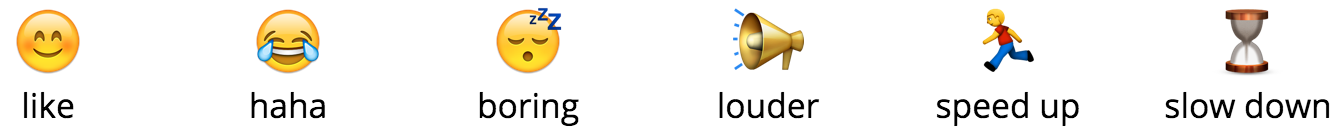
\includegraphics[width=.65\textwidth]{reactions}
\caption{All six possible reactions and their emoji (from left): \emph{approval}, \emph{laughter}, \emph{boredom}, \emph{louder}, \emph{speed up} and \emph{slow down}.}
\label{fig:design-reactions}
\end{figure}

\begin{figure}
\centering
\begin{tabular}{ccc}
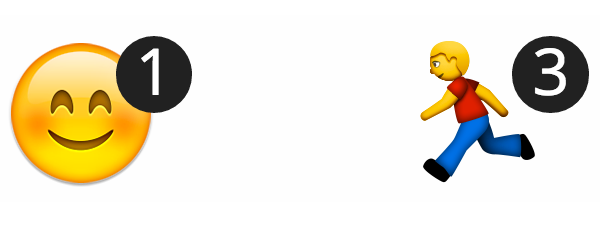
\includegraphics[width=.2\textwidth]{reactions-badge} &
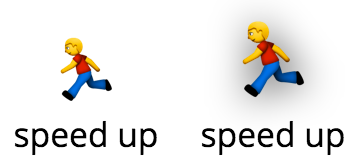
\includegraphics[width=.2\textwidth]{reactions-hover} \\
(a) & (b)
\end{tabular}
\caption{Details of visualisation of reactions (a) with number of reactions as found in the presenter view and optionally the projector and (b) reaction in listener interface with (right) and without hover-state (left).}
\label{fig:design-reactions-details}
\end{figure}

\section{Content Sharing}
% Sharing: show that it's possible to take photos on the phone directly!
% Explain muting
% Maybe use greg and amy again to show how greg copies a youtube link over or something
The last big module developed for the present thesis is the content sharing functionality. At the time of writing, the software allows for sharing photos (via links or from the computer or phone), websites, youtube videos and free text (including questions). In an earlier iteration, only one \emph{sharing} button was available in the interface, but feedback cycles with other web developers and designers have shown that it was not clear and intuitive enough which kind of content could be shared, which is why the functionality was now separated into three buttons: \emph{Media}, \emph{Link} and \emph{Question}. Coming back to Greg and Amy, Amy has just talked about functional programming and Greg wants to share a related video, of his favourite youtube channel funfunfunction\footnote{\url{https://www.youtube.com/channel/UCO1cgjhGzsSYb1rsB4bFe4Q}}. He opens the youtube app on his phone, searches for the video he wants to share and copies its link into the provided text field (see figure \ref{fig:design-sharing-youtube} (a)). When pressing the \emph{Share} button, Amy will receive a pop-up in which she can review the request and then accept it as a new main or subslide or dismiss it (see figure \ref{fig:design-sharing-youtube} (b)). If she accepts, the video will be inserted in a new slide relative to the slide Greg sent the request from. Youtube videos and links to websites are embedded into the presentation, similarly to images and links to images, which are also directly included into the created slide. Text is simply displayed as a second-order heading.

\begin{figure}
\centering
\begin{tabular}{ccc}
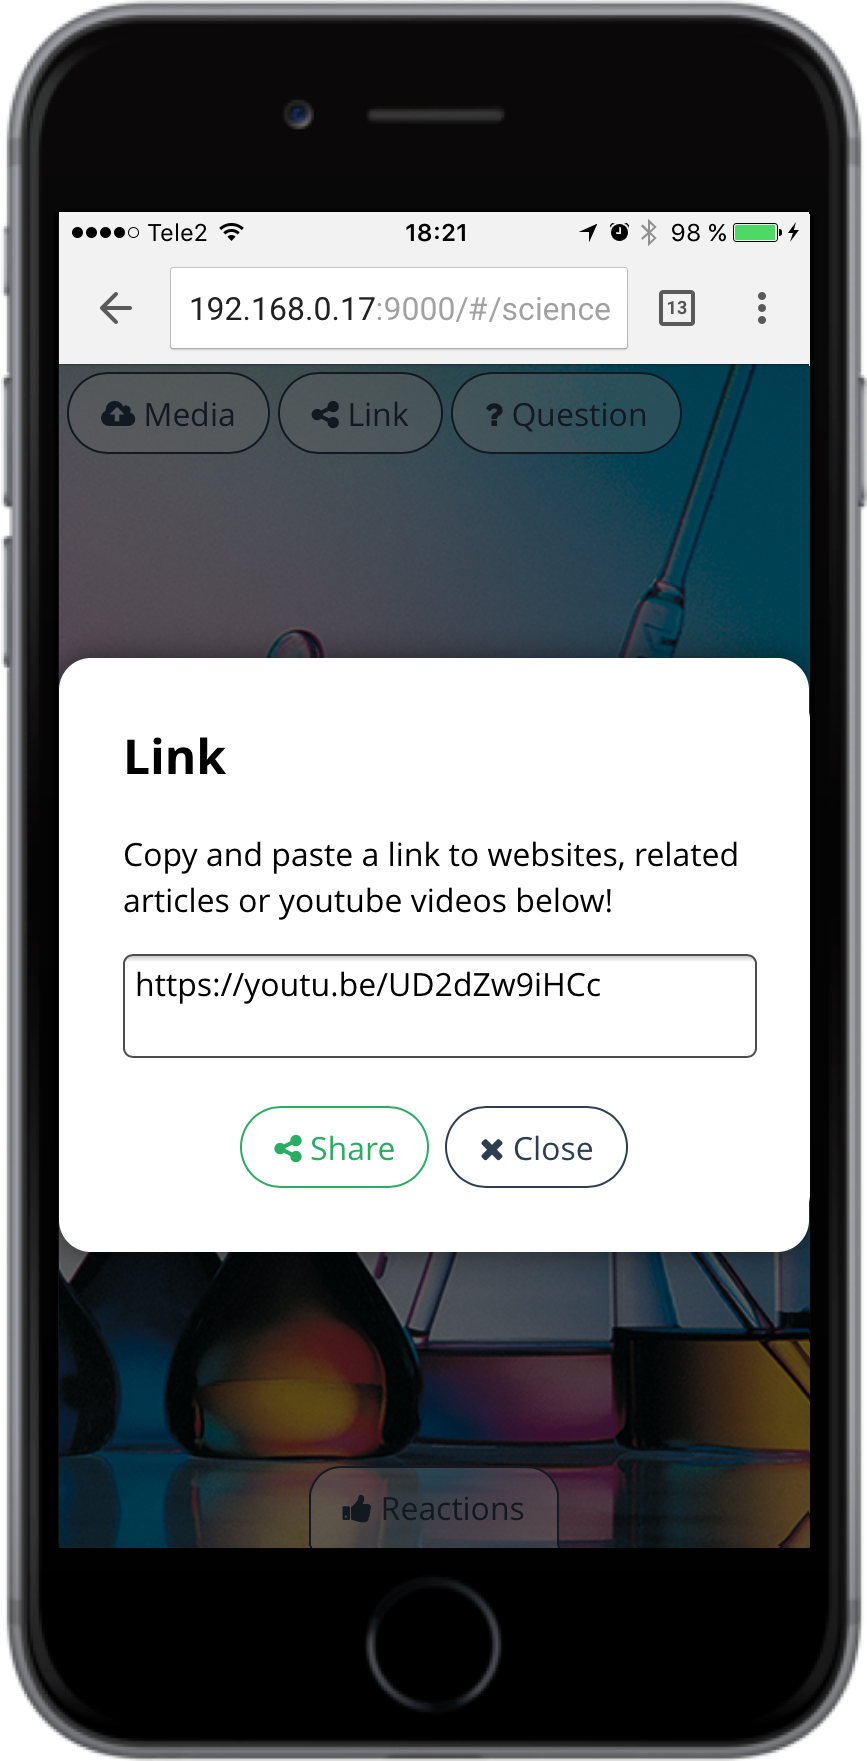
\includegraphics[width=.165\textwidth]{sharing-listener-youtube} &
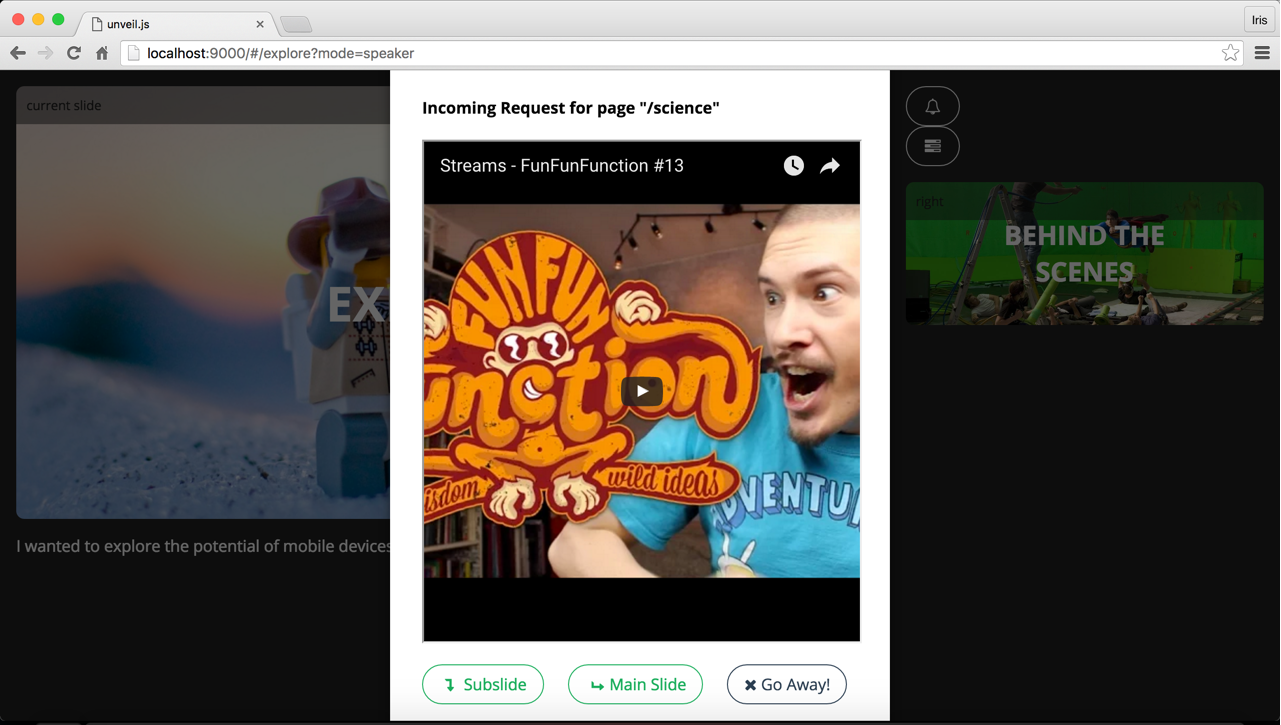
\includegraphics[width=.59\textwidth]{sharing-presenter-youtube} \\
(a) & (b)
\end{tabular}
\caption{Sharing of a youtube video. Request from listener on a phone (a) and accepting-modal in presenter-view on a computer (b).}
\label{fig:design-sharing-youtube}
\end{figure}

What was important to be able to include personal notes, is the ability to take photos and upload them to the presentation. This is possible in the \emph{Media} part of the content sharing feature (see figure \ref{fig:design-sharing-picture}) and makes use of the mobile operating system's native file uploads.

\begin{figure}
\centering
\begin{tabular}{ccc}
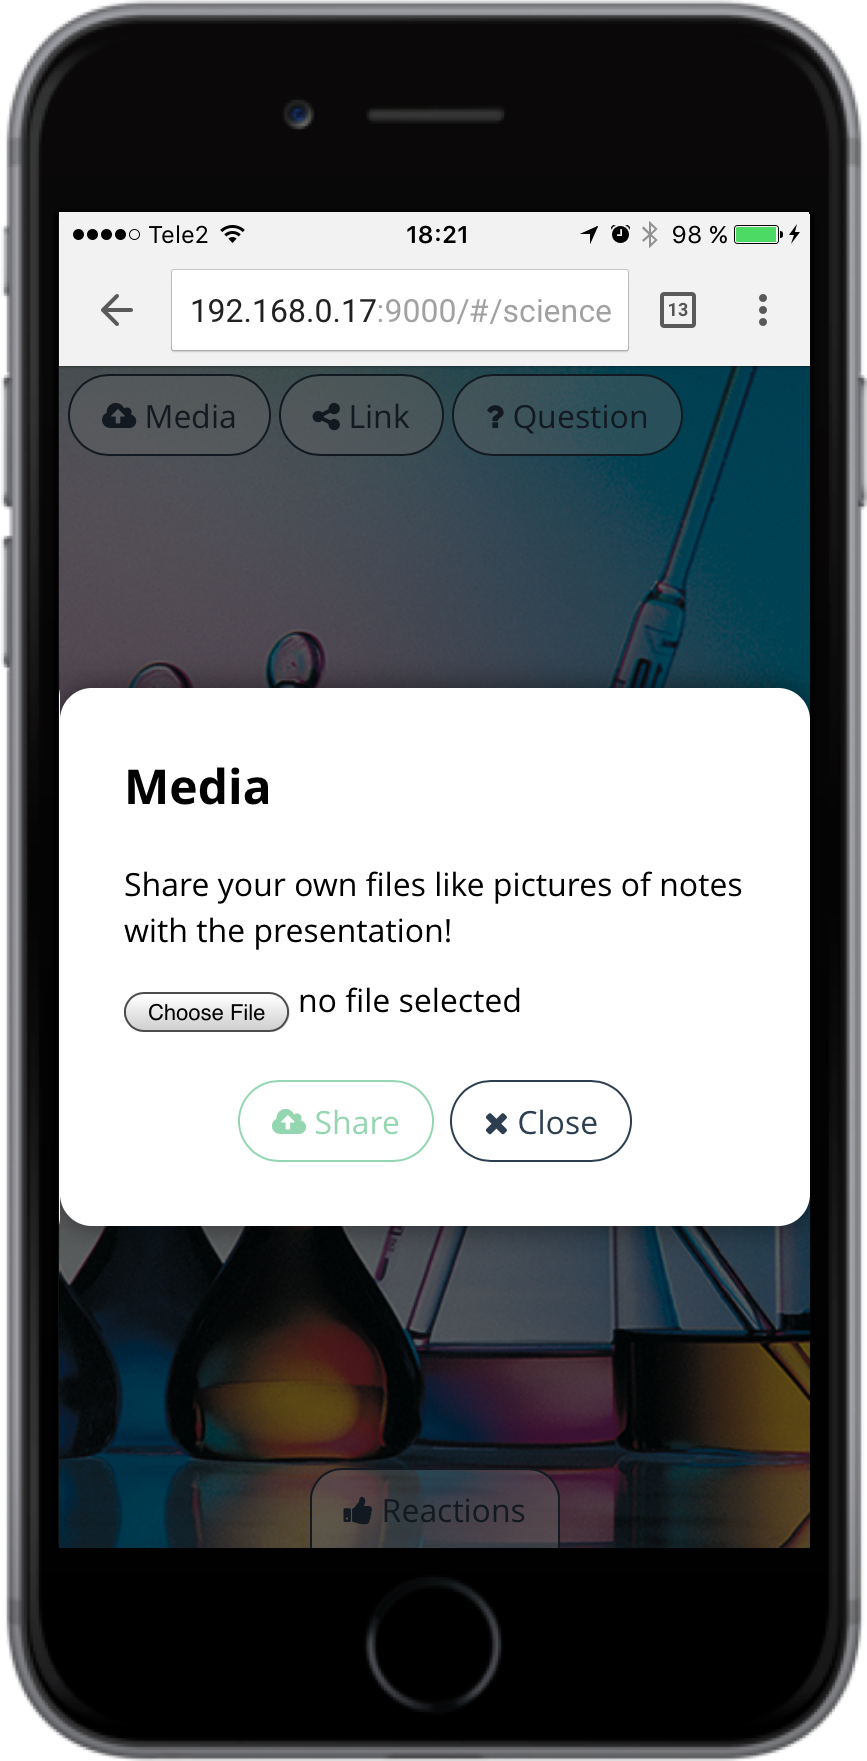
\includegraphics[width=.165\textwidth]{sharing-listener-1} &
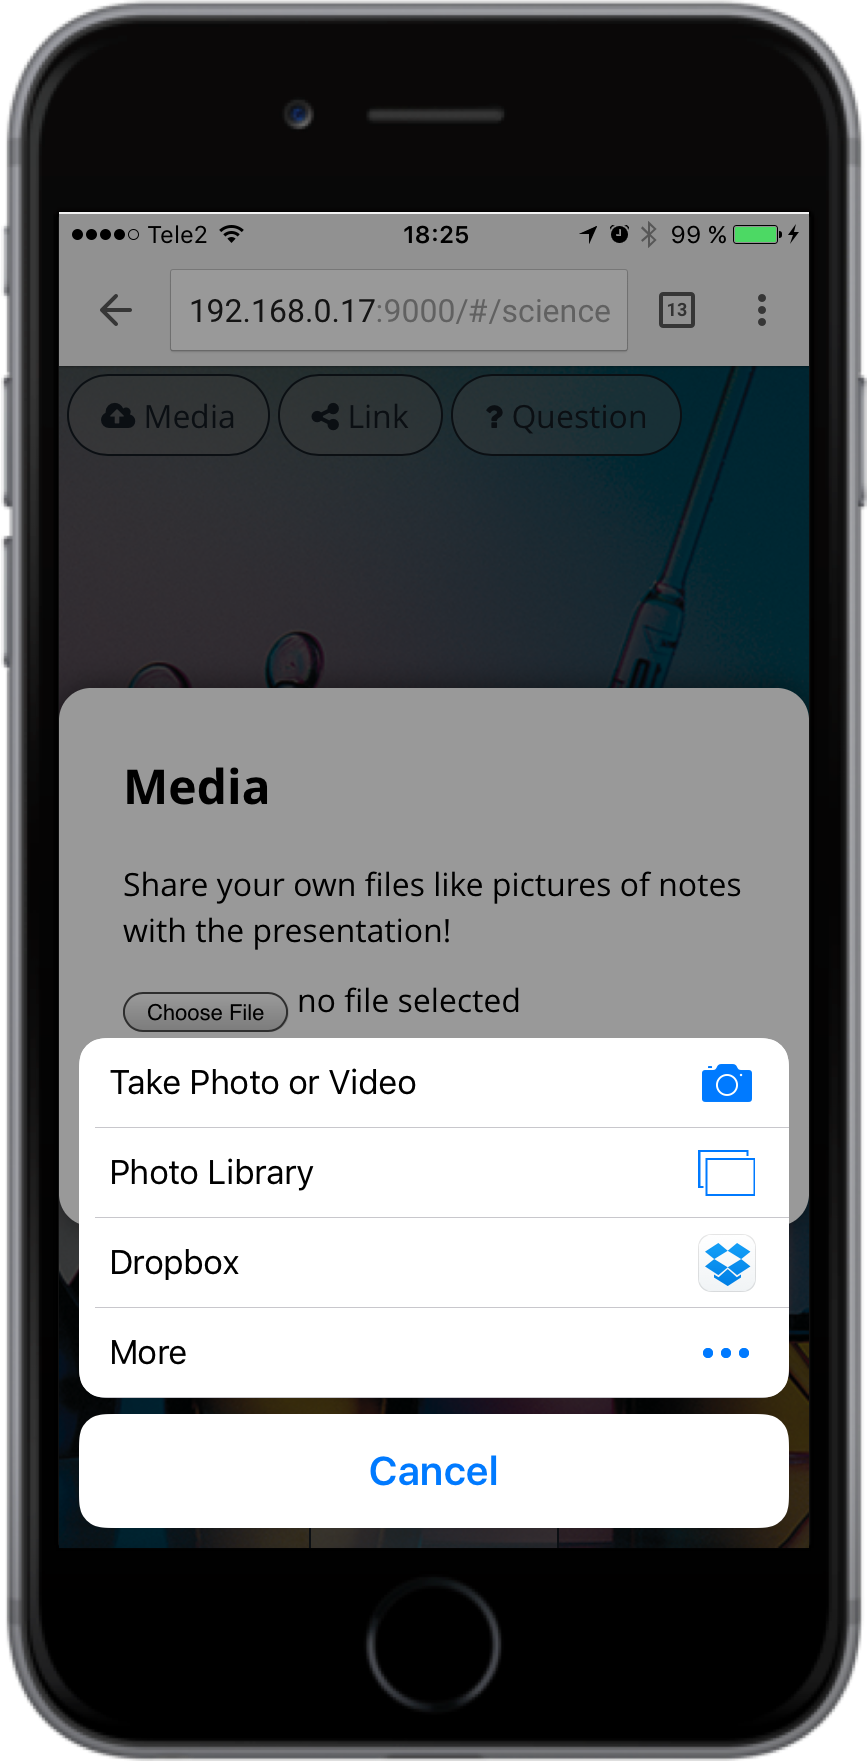
\includegraphics[width=.165\textwidth]{sharing-listener-2} &
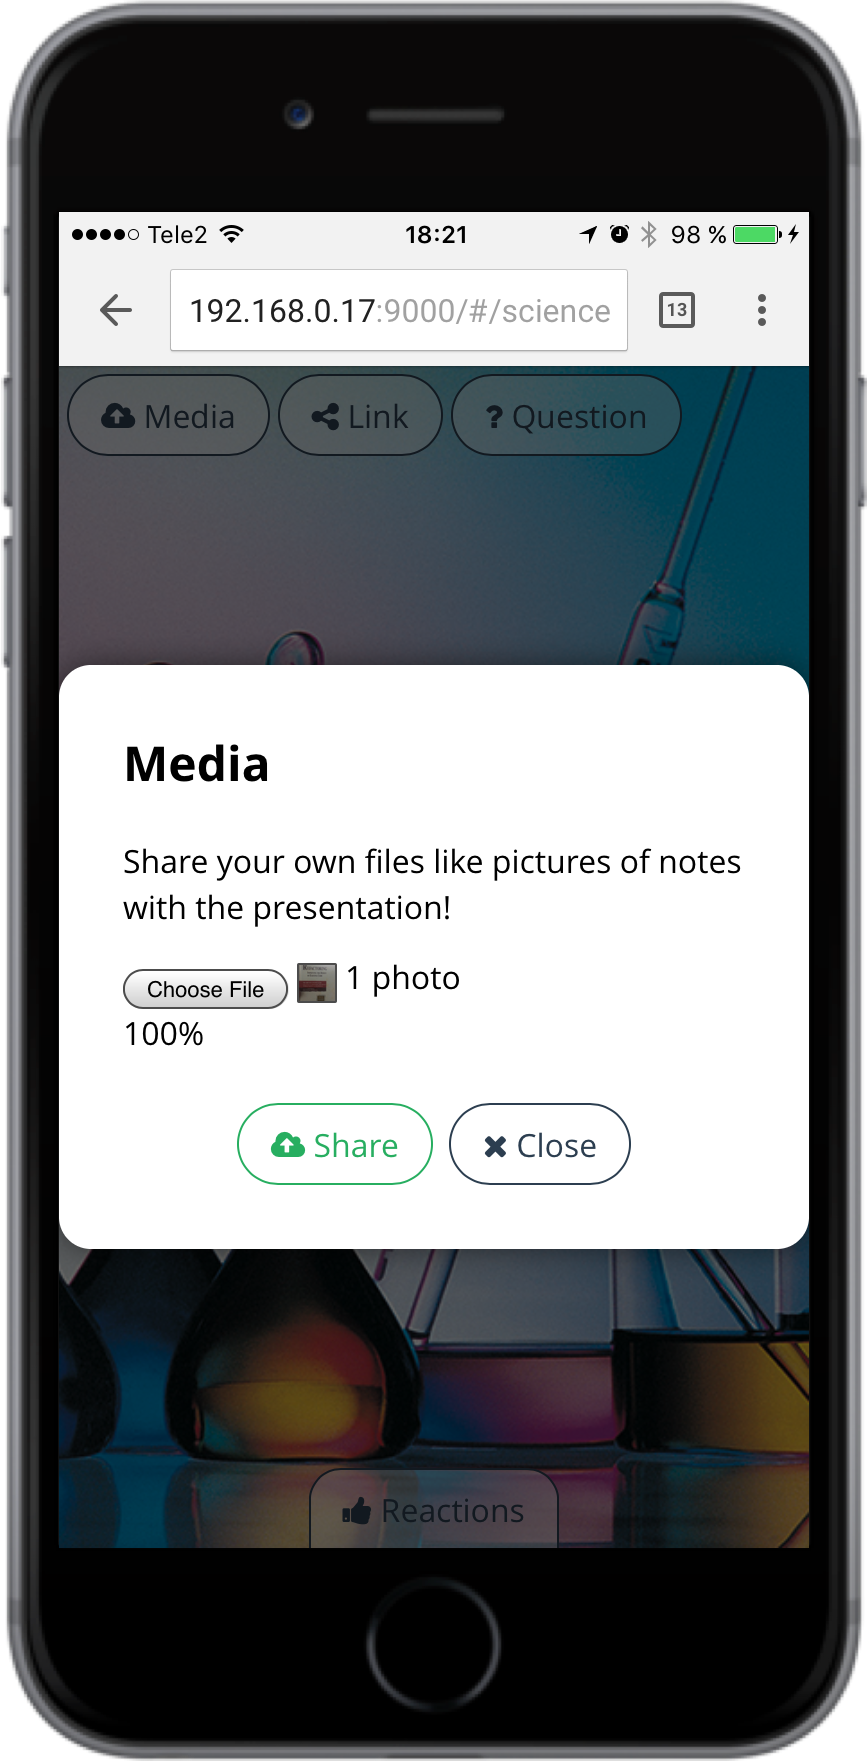
\includegraphics[width=.165\textwidth]{sharing-listener-3} \\
(a) & (b) & (c)
\end{tabular}
\caption{Sharing of a picture from an iPhone's browser (Google Chrome on iOS $9.3.4$) in listener mode. First, the listener opens the \emph{Media} sharing feature (a). Then a file can be chosen from different sources, such as the camera roll, or a new picture can be taken (b). In a last step, the picture is uploaded to the application and can then be shared (c).}
\label{fig:design-sharing-picture}
\end{figure}

Since such mechanisms can be fairly stressful for the presenter \cite{Teevan:MobileFeedbackDuringPresentation, Wacker:PresenterExperience}, we also built a feature to mute these requests. When muted, requests are automatically added as subslides to the slide the request was sent from, allowing all contributions to be collected without disturbing the flow of the presentation for the speaker \cite{Dieberger:NarrativeFlow}.

